\section{Results}

\subsection{Stationary data}

The stationary $C_y$ data obtained using flow simulations (Fig.\ref{cy ploynomial}(a))have a good agreement with data presented in \cite{Joly2012}. In comparison with the 7th order polynomial curve at \reynoldsnumber=22300 (Fig.\ref{cy ploynomial}(b))  several differences could be observed. The peak value of $C_y$ is  significantly low at \reynoldsnumber=165 ($C_y=0.05$ at $4^0$) in comparison with \reynoldsnumber=22300 ($C_y=0.57$ at $13^0$) . The inflection point present at \reynoldsnumber=22300 could not be observed at \reynoldsnumber=165. This agrees with the findings of \cite{Luo2003}. It was concluded by \cite{Luo2003} that hysteresis occur due to the inflection point found in the $C_y$ curve. Therefore hysteresis is not expected at \reynoldsnumber=165. The range of the incident flow angles where $C_y$ remain positive is narrow at \reynoldsnumber=165 ($0^0 <\theta \leq$ $6^0$) compared to \reynoldsnumber=22300 ($0^0 <\theta \leq 15^0$). This feature is what sustains galloping and power is transferred from the fluid to the supporting structure within this range of incident angle because fluid forces are acting in the direction of travel of the oscillating cylinder. Incident angles beyond this range actually suppresses the galloping and power goes in the opposite direction. Therefore due to the overall smaller $C_y$ and narrow range of angles where $C_y$ is positive for \reynoldsnumber=165 compared to \reynoldsnumber=22300 leads one to expect a significant reduction in power at\reynoldsnumber=165 compared to \reynoldsnumber=2230.

  

\begin{figure}
  \setlength{\unitlength}{\textwidth}

  \begin{picture}(1,0.72)
%(0,0.35)
    
    % % %Parkinson Data 
    \put(0.025,0.48){\includegraphics[width=0.5\unitlength]{../FnP/gnuplot/displacement_amp_re_parkinson_1.eps}}
    \put(0.025,0.25){\includegraphics[width=0.5\unitlength]{../FnP/gnuplot/velocity_amp_re_parkinson.eps}}
    \put(0.025,0.02){\includegraphics[width=0.5\unitlength]{../FnP/gnuplot/mean_power_re_parkinson.eps}}
    
    % Re 165 Data 
    \put(0.495,0.48){\includegraphics[width=0.5\unitlength]{../FnP/gnuplot/displacement_amp_re165.eps}}
    \put(0.495,0.25){\includegraphics[width=0.5\unitlength]{../FnP/gnuplot/velocity_amp_re165.eps}}
    \put(0.495,0.02){\includegraphics[width=0.5\unitlength]{../FnP/gnuplot/mean_power_re_165.eps}}
   
%    \put(0.25,0.93){\ustar}
%    \put(0.8,0.93){\ustar}
%    \put(0.25,0.63){\ustar}
%   \put(0.8,0.63){\ustar}
    \put(0.25,0.0){\ustar}
    \put(0.75,0.0){\ustar}
    
    \put(0.00,0.6){$\displaystyle\frac{A}{D}$}
%    \put(0.52,1.075){$\frac{A}{D}$}
    \put(0.00,0.4){$\displaystyle\frac{V}{D}$}
%    \put(0.52,0.83){$\frac{V}{D}$}
    \put(-0.025,0.15){$\displaystyle\frac{P_{m}}{\rho \mathcal{A}U^3 }$}
%    \put(0.5,0.54){$\frac{P_{m}}{\rho \mathcal{A}U^3 }$}
    
    \put(0.085,0.685){\small(a)}
    \put(0.555,0.685){\small(b)}
    \put(0.085,0.455){\small(c)}
    \put(0.555,0.455){\small(d)}
    \put(0.085,0.225){\small(e)}
    \put(0.555,0.225){\small(f)}   
  \end{picture}

%  \vspace{-4cm}
  \caption{Velocity amplitude, displacement amplitude and mean power  as functions of $U^*$. Data presented in (a), (c) and (e) were calculated using input data at $Re=22300$ and $m^*=1163$ obtained by \cite{Parkinson1964} at three different damping ratios: $\zeta=0.0125$ (\ding{83}), $\zeta=0.015$ (\ding{116}) and $\zeta=0.0175$ (\ding{108}). Data presented in (b),(d) and (f) were obtained using input data at $Re=165$ and $m^*=20$ at three different damping ratios: $\zeta=0.075$ ($\times$), $\zeta=0.1$ (\ding{117}) and $\zeta=0.15$ (+). The multiple branches for the higher Re are due to the hysteresis between two solutions.}
  
\label{fig:uncollapsed_data}
\end{figure}




\subsection{Displacement,velocity and power output as a function of reduced velocity}


 The quasi-steady analysis data reveals that the displacement amplitude tend to grow with increasing $U^*$ Fig.\ref{fig:uncollapsed_data} (a) and (b). The onset of galloping is delayed with increasing $\zeta$ for both high and low Reynolds numbers. This echo the findings of previous studies by \cite{Parkinson1964} and \cite{Barrero-Gil2010a}. Hysteresis could be observed for the case with a higher Reynolds number. This was achieved by manipulating the initial conditions (initial displacement) of the system. The upper branch was obtained by giving an initial displacement which was higher than the expected amplitude while the lower branch was obtained by providing a lower initial displacement than the expected amplitude. Although a third state could be achieved theoretically, it was not possible to achieve numerically. This was also observed by \cite{Vio2007}.   

 
 \subsubsection*{Power vs $U^*$}
 
 The mean power grows, peaks and then reduces as $U^*$ is increased (Fig.\ref{fig:uncollapsed_data} (e) and (f)) for each value of $\zeta$. The value of \ustar at which the peak power occurs increases with $\zeta$. However, the magnitude of the peaks remain constant for all the values of $\zeta$.  \cite{Barrero-Gil2010a} also showed a similar trend. The higher Reynolds number case clearly showed hysteresis in the power data. The range of hysteresis tend to increase with increasing $\zeta$. It could be observed that unlike VIV the  system has no preferred frequency. Although the onset of galloping and the point where peak power occur at different $U^*$ when the damping ratio is changed, the peak power remains constant regardless of $U^*$.
 
 \subsection{Galloping response and natural frequency}
 
 Now the oscillator equation Eq.\eqref{final_equation_motion} is considered from a power perspective. The shedding forces can be neglected because the net effect is negligible as system oscillates at natural frequency which is far from shedding frequency, for the cases that exhibit galloping. It is obvious that the forcing term on LHS of the equation is only dependent on transverse velocity($\dot{y}$) which is essentially the input power of the system. On the RHS, the mechanical damping or system damping is the only term that takes out power at any instant. This could be expressed as the product of damping force and the velocity ($P_d$). The inertia and the stiffness terms governs the frequency of the system but the forces associated by those terms are conservative forces (i.e there is zero net energy in or out of the system when averaged over a period). Therefore the system is governed by the transverse velocity rather than the natural frequency.
 

 Using $U^*$ and $\zeta$ assumes that the system has a preferred frequency because they scale with the natural frequency of the system. The effect of fixing $\zeta$ and increasing $U^*$ actually decreases the damping constant for a fixed free-stream velocity. ($U^*=\frac{U}{f \times D}$, $\zeta= \frac{c}{2 m \omega_n}$ ). Both these effects leads to the multiple lines that are horizontally transpose when $\zeta$ is increased (Fig.\ref{fig:uncollapsed_data} (e) and (f)). Therefore the effect of $\zeta$ essentially scales up the damping coefficient for a fixed $U^*$.
 
 The data presented in Fig.\ref{fig:uncollapsed_data} for various damping ratios ,$\zeta$, can be collapsed into a single line for a for a particular force characteristic curve (i.e $C_y$ vs $\theta$ curve)  curve could be obtained for the velocity amplitude  and power were plotted as a function of  non dimensionalised  damping constant $c\rho\mathcal{A}U$ 
(Fig \ref{fig:collpased_data} (a),(b),(c) and (d)).  This further emphasizes that the galloping system is not frequency dependent. It is possible to obtain a different similar power output at different values of \ustar when the damping constant, $c\rho\mathbb{A}U$, is kept fixed. An example of this case, as shown in Fig.\ref{fig:time_hostory_velocity_same_power}, clearly show that this is a result of similar velocity amplitudes between cases if one were to disregard the high frequencies due to shedding. As mentioned earlier, it is the transverse velocity that determines the energy provided by the fluid forcing and the mechanical damping.

\begin{figure}
  \setlength{\unitlength}{\textwidth}

        \begin{picture}(1,0.74)

      % % % Parkinson Data 
      \put(0.025,0.5){\includegraphics[width=0.5\unitlength]{../FnP/gnuplot/displacement_amp_collapsed_parkinson.eps}}
      \put(0.025,0.27){\includegraphics[width=0.5\unitlength]{../FnP/gnuplot/velocity_amp_collapsed_parkinson.eps}}
      \put(0.495,0.27){\includegraphics[width=0.5\unitlength]{../FnP/gnuplot/velocity_amp_collapsed_re165.eps}}
      
      \put(0.025,0.02){\includegraphics[width=0.5\unitlength]{../FnP/gnuplot/mean_power_collapsed_parkinson.eps}}
      \put(0.495,0.02){\includegraphics[width=0.5\unitlength]{../FnP/gnuplot/mean_power_collapsed_re_165.eps}}
      \put(0.495,0.5){\includegraphics[width=0.5\unitlength]{../FnP/gnuplot/displacement_amp_collpased_re165.eps}}
      
      \put(0.23,0.00){ $\displaystyle\frac{c}{\rho\mathcal{A}U}$}
      \put(0.73,0.00){ $\displaystyle\frac{c}{\rho\mathcal{A}U}$}
      
      \put(0.01,0.405){$\displaystyle\frac{V}{D}$}\
       \put(0.01,0.63){$\displaystyle\frac{A}{D}$}
      
      \put(-0.02,0.13){$\displaystyle\frac{P_{m}}{\rho \mathcal{A}U^3 }$}
      
      \put(0.46,0.709){\small(a)}
      \put(0.93,0.709){\small(b)}
      \put(0.46,0.475){\small(c)}
      \put(0.93,0.475){\small(d)}
      \put(0.46,0.225){\small(e)}
      \put(0.935,0.225){\small(f)}
      
    \end{picture}

  \caption{Displacement amplitude, velocity amplitude and mean power as functions of the damping factor. Data presented in (a),(c) and (e)  were calculated using input data at $Re=22300$ obtained by \cite{Parkinson1964} at three different damping ratios: $\zeta=0.0125$ (\ding{83}), $\zeta=0.015$ (\ding{116}) and $\zeta=0.0175$ (\ding{108}). Data presented in (b), (d) and (f)  were obtained using input data at $Re=165$ at three different damping ratios: $\zeta=0.075$ ($\times$), $\zeta=0.1$ (\ding{117}) and $\zeta=0.15$ (+). The collapsed data implies that there is no frequency selection and the tuning parameter of the mechanical side of the system is the damping constant to obtain an optimum power output.}
    \label{fig:collpased_data}
\end{figure}

 %vspace{10cm}

 
\begin{figure}
  \setlength{\unitlength}{\textwidth}
  \begin{picture}(1,0.3)(0,0.8)
    % % %90
    \put(0.025,0.83){\includegraphics[width=0.5\unitlength]{../FnP/gnuplot/vel_time_history_60_0.075.eps}}
    \put(0.495,0.83){\includegraphics[width=0.5\unitlength]{../FnP/gnuplot/vel_time_history_165_0.175.eps}}
    
    \put(0.03,0.95){ $\frac{V}{D}$} 	
    % \put(0.56,1.02){ $\frac{V}{D}$}
 	
    \put(0.25,0.805){ $\frac{tU}{D}$} 	
    \put(0.73,0.805){ $\frac{tU}{D}$}

    \put(0.095,1.03){(a)}
    \put(0.565,1.03){(b)}

  \end{picture}

  \caption{Time histories of velocity at two different $\zeta$ and $U^*$ which produce the same mean power ($1.2\times10^{-3}$). Data presented in (a) are at $\ustar=60$, $\zeta=0.075$ and (b) are at $\ustar=165$, $\zeta=0.175$. Both data sets were obtained using Quasi-steady state assumption using input $C_y$ parameters at $Re=165$. Shedding is evident in both signals as a high frequency fluctuation but the amplitude of the slower fluctuations remains constant in both cases.}
    \label{fig:time_hostory_velocity_same_power}
\end{figure}

 


 
 Power could be expressed as the product of force and velocity. Therefore the transferred power form fluid-to-body could be expressed as $P_t=F_y\dot{y}$. Similarly the dissipated power due to the mechanical damping could be expressed as $P_d=(c\dot{y})\dot{y}$. The time average of these two quantities should be equal due to energy conservation, provided that the mechanical friction is neglected . Analysing the  time histories of $P_t $ and $P_d$ at key regions (Fig.\ref{fig:regions_1}) on the mean power vs $U^*$ provides a detailed explanation for the variation of the output powe when the reduced velocity is increased. The key regions consists of region 1 where the $P_m$ increases with \ustar, region 2 where $P_m$ becomes maximum and region 3 where $P_m$ decreases with \ustar. It has been established earlier that the damping factor is a function of $U^*$. Therefore it could be derived that $U^*$ is inversely proportional to damping coefficient. Hence the damping coefficient reduces when you move from region 1 to 3.Fig \ref{fig:lift_curves} (a) shows that $C_y$ and therefore instantaneous force rises until $4^0$ where it peaks and then falls and at around $6^0$ becomes negative. Maximum amount of power could be transferred within the peak region. At the region where the instantaneous force becomes negative it will be opposing the velocity $\dot{y}$.Data at $\zeta=0.1$, $m^*=40$ and \reynoldsnumber=165 (Fig.\ref{fig:power_time_histories}) are analysed as and example.  

\begin{figure}[h!]
\centering
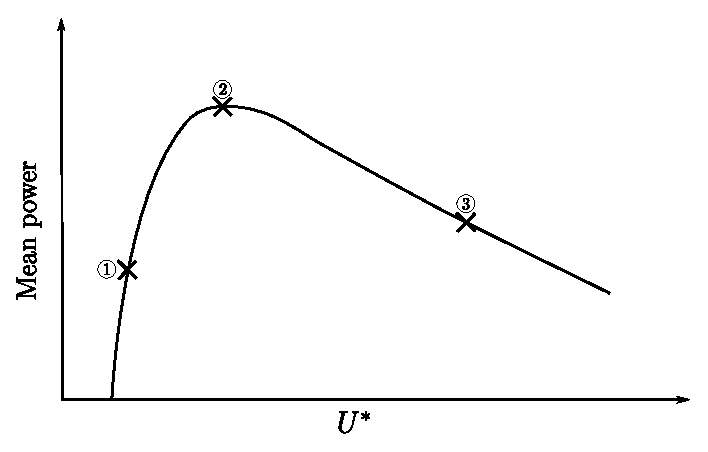
\includegraphics[width=0.5\textwidth]{../FnP/sketch_1}
\caption{ Three key regions taken into account to analyse the time histories of power in a typical mean power vs. $U^*$ curve at $Re=165$. In region 1, high damping suppresses oscillation, hence the power output is low. In region 2, the damping is close to the optimum for power transfer. In region 3, the low damping means little energy is extracted from the fluid.}
\label{fig:regions_1}
\end{figure}

 
 
 
 At region 1 where $U^*=90$ the damping constant is high and a clear sinusoidal signal could be observed for both $P_d$ and $P_t$ in Fig. \ref{fig:power_time_histories} (a). Fig.\ref{fig:power_time_histories} (d) and (g) shows that $\theta$ is in line or in phase with $F_y$.  The velocity amplitude in this case is small and the equivalent incident angle within the range where the hydrodynamic force increases with the incident angle (i.e. $0<\theta \leq < 4^0$ in \ref{fig:lift_curves}) Hence both $P_d$ and $P_t$ becomes sinusoidal. In this case, power output is limited by the low fluid forces present at low incident angles. In other words damping is significantly high and extracts a lot of power that the velocity amplitude could not grow where the forcing  is significant to produce high level of power.   
 
 
  At region 3 ($U^*= 400$) `$c$' is low in comparison with region 1 and 2 which leads to a low mean power output. Fig.\ref{fig:power_time_histories} (c) shows that $P_t$ becomes negative over some portion of the cycle. This is because $\theta$  passes the point where both $\theta$ and $C_y$ (therefore $F_y$) are positive. The high velocity amplitude leads to the equivalent incident angle $\theta$, in this case to exceed the range where $C_y$ is positive (i.e. $0<\theta<6^0$ in Fig.\ref{cy ploynomial} (a)). In this portion of the cycle the hydrodynamic force actually opposes the direction of travel and power is transferred from the structure to the fluid during those times. From and energy perspective, the mechanical damping is not sufficient to remover the energy transferred from the fluid to the structure during other times of the cycle because $c\rho\mathcal{A}U$ is substantially low. Therefore this excess energy is transferred back to the fluid as depicted by the negative region of $P_d$ in \ref{fig:power_time_histories} (c) 
 

At region 2 ($U^*=165$). $P_t$ is not a pure sinusoidal signal. However, the  signal remains periodic. From the time history graph of $P_t$, two `peaks' are present in a single half cycle (Fig \ref{fig:power_time_histories} (b)). In this case, the velocity amplitude actually exceeds the equivalent incident angle where the hydrodynamic forces peaks (i.e. $\theta=4^0$ in \ref{cy ploynomial} (a)). The dips in $P_d$ between the two peaks approximately correspond to the time where the transverse velocity is higher than 0.07 and $F_y$ is decreasing with increasing transverse velocity. The mean power output is at its maximum. This is due to the fact that this region is a best compromise between region 1 and 3. The damping is substantially high to obtain a high power output while not too high to hinder the induced angle of attack entering the region where the forcing is high. 


 
  
\begin{figure}

  \setlength{\unitlength}{\textwidth}
%  \fbox{
  \begin{picture}(1,0.58)(0,0.35)
    % % % 90
    \put(0.03,0.76){\includegraphics[width=0.35\unitlength]{../FnP/gnuplot/power_time_history_90.eps}}
    \put(0.03,.58){\includegraphics[width=0.35\unitlength]{../FnP/gnuplot/f_y_history_90.eps}}
    \put(0.03,0.4){\includegraphics[width=0.35\unitlength]{../FnP/gnuplot/theta_time_history_90.eps}}
    
    % % 165
    \put(0.36,0.76){\includegraphics[width=0.35\unitlength]{../FnP/gnuplot/power_time_history_165.eps}}
    \put(0.36,.58){\includegraphics[width=0.35\unitlength]{../FnP/gnuplot/f_y_history_165.eps}}
    \put(0.36,0.4){\includegraphics[width=0.35\unitlength]{../FnP/gnuplot/theta_time_history_165.eps}}
    
    \put(0.68,0.76){\includegraphics[width=0.35\unitlength]{../FnP/gnuplot/power_time_history_400.eps}}
    \put(0.68,.58){\includegraphics[width=0.35\unitlength]{../FnP/gnuplot/f_y_history_400.eps}}
    \put(0.68,0.4){\includegraphics[width=0.35\unitlength]{../FnP/gnuplot/theta_time_history_400.eps}}
    
    \put(0.55,0.36){$\displaystyle{\frac{tU}{D}}$}
    \put(0.2,0.36){$\displaystyle{\frac{tU}{D}}$}
    \put(0.85,0.36){$\displaystyle{\frac{tU}{D}}$}
    
    \put(0.0,0.87){$\frac{P}{\rho \mathcal{A}U^3}$}
    \put(0.01,0.66){$F_y$}
    \put(0.01,0.49){$\theta$}
    
    \put(0.08,0.76){(a)}
    \put(0.08,0.58){(d)}
    \put(0.08,0.38){(g)}
    
    \put(0.4,0.76){(b)}
    \put(0.4,0.58){(e)}
    \put(0.4,0.38){(h)}
    
    \put(0.72,0.76){(c)}
    \put(0.72,0.58){(f)}
    \put(0.72,0.38){(i)}
  \end{picture}
%}
  \caption{Time histories of $P_t$, $P_d$, $F_y$ and $\theta$ at $\ustar=90$, $165$ and $400$. Data was obtained at $\zeta=0.1$, $m^*=40$ and \reynoldsnumber=165. The time histories of $P_t$ ( \solidrule[4mm]\hspace{1mm}) and $P_d$ (\protect\dashedrule) are presented for: (a) $\ustar = 90$; (b) $\ustar = 165$; (c) $\ustar = 400$. Time histories of the instantaneous force $F_y$ for: (d) $\ustar = 90$; (e $\ustar = 165$; (f) $\ustar = 400$. Time histories of the instantaneous angle $\theta$ for: (g) $\ustar = 90$; (h) $\ustar = 165$; (i) $\ustar = 400$.}
  \label{fig:power_time_histories}
\end{figure}





 



\subsection{Effect of $m^*$}

 \begin{figure}

\setlength{\unitlength}{\textwidth}
\fbox{
  \begin{picture}(1,0.32)
    
       \put(0.07,0.03){\includegraphics[width=0.3\unitlength]{../FnP/gnuplot/mean_power_collapsed_mstar.eps}}
       \put(0.36,0.03){\includegraphics[width=0.3\unitlength]{../FnP/gnuplot/mean_power_collapsed_noshed_mstar.eps}}
       \put(0.65,0.03){\includegraphics[width=0.3\unitlength]{../FnP/gnuplot/fsi_power.eps}}
        
        \put(0.03,0.17){\large $\frac{P_{m}}{\rho \mathcal{A}U^3}$}
              
        \put(0.2,0.0){$\frac{c}{\rho\mathcal{A}U}$} 	
        \put(0.49,0.0){$\frac{c}{\rho\mathcal{A}U}$}
        \put(0.78,0.0){$\frac{c}{\rho\mathcal{A}U}$}
    
        \put(0.133,0.21){\small(a)}
        \put(0.42,0.21){\small(b)}
        \put(0.715,0.21){\small(c)}
    
 

     

  \end{picture}
  }

  \caption{Mean power as a function of damping factor. Data are presented at $m^*=10$ (\ding{108}), $m^*=20$ (\ding{83}), $m^*=40$ (\ding{115}), $m^*=60$ (+) at Re 165 and $\zeta=0.1$. A reduction of maximum mean power can be observed when $m^*<40$. For $m^*>40$, the maximum power is essentially independent of $m^*$.}
    \label{fig:m_star_collapsed}
\end{figure}



Mean power as a function of damping factor at Re

The maximum mean power at different $m^*$ (Fig.\ref{fig:m_star_collapsed}) was constant beyond $m^*=30$. However, at $m^* \leq 30$ an effect of $m^*$ it could be observed. Not only the peak value but overall reduction in the mean power could be observed when $m^*$ was reduced.When galloping excitation is suppressed al low $m^*$, the system will exhibit a weak response as a result of forcing from vortex shedding. This was also reported by \cite{Joly2012} where galloping amplitude was reduced at low $m^*$. The suppression of galloping as $m^*$ is reduced can be explained by looking at the difference between the instantaneous power transfer between fluid to the structure $P_t$ and the power taken out by the mechanical damping $P_t$ in \ref{fig:power_time_histories}. While the time avergae of both quantities are the same, instantaneously they are not. Therefore the mechanical system is required to store power in certain points of the cycle and release it at another portion of the cycle. In cases where $m^*$ is very low, the system lack adequate inertia to store this power which leads to suppression of galloping. 

 \begin{figure}
  \setlength{\unitlength}{\textwidth}
  \begin{picture}(1,0.25)
    % % %90
    \put(0.02,0.03){\includegraphics[width=0.3\unitlength]{../FnP/gnuplot/fsi_displacement.eps}}
    \put(0.36,0.03){\includegraphics[width=0.3\unitlength]{../FnP/gnuplot/fsi_velocity.eps}}
    \put(0.72,0.03){\includegraphics[width=0.3\unitlength]{../FnP/gnuplot/fsi_power.eps}}
    
    \put(0.02,0.15){$\displaystyle\frac{A}{D}$}
    \put(0.35,0.15){$\displaystyle\frac{V}{D}$}
    \put(0.67,0.15){$\displaystyle\frac{P_{m}}{\rho \mathcal{A}U^3 }$}
    
    \put(0.18,0.01){\ustar} 	
    \put(0.51,0.01){\ustar}
    \put(0.87,0.01){\ustar}

    \put(0.092,0.21){\small(a)}
    \put(0.42,0.21){\small(b)}
    \put(0.78,0.21){\small(c)}

  \end{picture}  

  \caption{Comparison of data generated using the quasi-static theory (\ding{83}) and full DNS simulations (\ding{108}). (a) Displacement amplitude, (b) velocity amplitude and (c) mean power as functions of \ustar. Data were obtained at $Re=165$ and $\zeta=0.075$. An average difference of $34\%$ is observed for both displacement and velocity amplitude. However, the essential physics i.e the rise and fall of mean power, is captured by DNS simulations.}
    \label{fig:FSI_QSS_compare}
\end{figure}

\subsection{Comparison with FSI simulations}
 Similar trends were captured for both displacement and velocity amplitudes between QSS and FSI simulations (Fig. \ref{fig:FSI_QSS_compare}(a) and \ref{fig:FSI_QSS_compare}(b)). Quantitatively a large discrepancy (average of $30\%$) could be observed between QSS and FSI data. Therefore the power also becomes significantly low in FSI data (Fig.\ref{fig:FSI_QSS_compare}(c)). However, the FSI data (Fig.\ref{fig:FSI_QSS_compare} (c)) were able to produce the main the rise and the fall of mean power when $U^*$ was increased. The reasoning behind this fact is that galloping is weak at Re 165  and therefore fluid damping has a significant effect. It was reported by \cite{Barrero-Gil2009} that galloping only starts to occur ar Re $\geq 159$. As power is function of $(\dot{y})^2$ the error between QSS and FSI power becomes significantly large.  
 

 

\section{Conclusion}








 

 
 
 

 
 


 % % % % % % % % % % % % % % % % % % % % % % % % % % % % % % % % % % % % % % % % %

 
 
 
 
 
 
 
 
 
 
  
 
 
